\begin{flushright} {\tiny {\color{gray} python\_codes/fieldstone\_115/text.tex}} \end{flushright}

%\lstinputlisting[language=bash,basicstyle=\small]{python_codes/fieldstone_01/keywords}

\begin{center}
\fbox{\textbf{\huge \color{teal} P}}
Codes at \url{https://github.com/cedrict/fieldstone/tree/master/python_codes/fieldstone_115}
\end{center}

\par\noindent\rule{\textwidth}{0.4pt}

%%%%%%%%%%%%%%%%%%%%%%%%%%%%%%%%%%%%%%%%%%%%%%%%%%%%%%%%%%%%%%%%%%%%%%%%%%%%%%%%%%%%%%%%%%%%%%


Big questions

- how to deal with vicosity contrasts ? 

- which stab is best ? 

- how to deal with not square mesh ?


Theory is explained in Section~\ref{ss:pairq1p0stab}.


%-------------------------------------------
\subsection*{Penalty approach}

The $\C$ matrix is actually diagonal so that the sparsity pattern of the matrix is as follows:
\begin{center}
\includegraphics[width=7cm]{python_codes/fieldstone_115/results/nostab/matrix}
\includegraphics[width=7cm]{python_codes/fieldstone_115/results/penalty/matrix}\\
{\captionfont Sparsity pattern of regular element (keft), and penalty-'stabilised' element(right).}
\end{center}

We find that the presence of the $\C$ matrix is enough to suppress the chequerboard mode:
\begin{center}
\includegraphics[width=6cm]{python_codes/fieldstone_115/results/nostab/press}
\includegraphics[width=6cm]{python_codes/fieldstone_115/results/penalty/press}\\
{\captionfont 32x32. Left: no stabilisation. Right: penalty stabilisation with $\epsilon=10^{-6}$}
\end{center}

We can now explore the influence of the stabilisation parameter $\epsilon$. Obviously, 
if too low it won't have any effect as the $\C$ matrix then tends to zero. If too high,
then we expect it to perturb the solution too much. 
The pressure field is shown in the following figure for various values of $\epsilon$, 
and no pressure normalisation is implemented at all. We find that not only the 
penalty stabilisation removes the chequerboard mode but it also automatically 
normalises the pressure...?  

\begin{center}
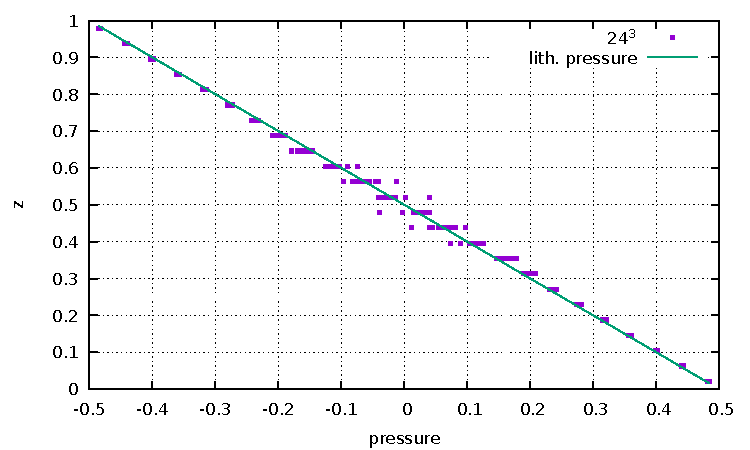
\includegraphics[width=9cm]{python_codes/fieldstone_115/results/pressure.pdf}\\
{\captionfont 32x32. influence of $\epsilon$ parameter} 
\end{center}

Let us now turn to the error convergence rates after carrying out a pressure normalisation 
as a postprocessor:
\begin{center}
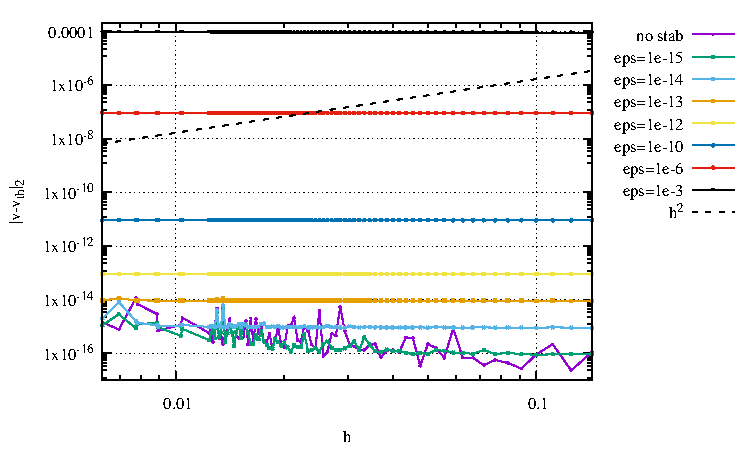
\includegraphics[width=8cm]{python_codes/fieldstone_115/results/errorsV_penalty.pdf}
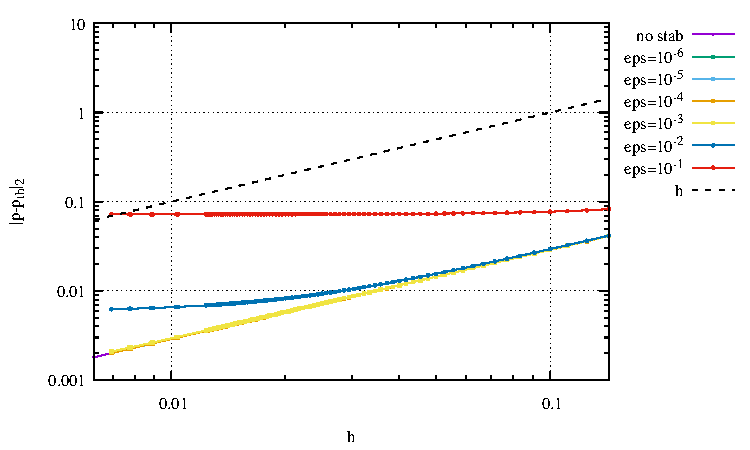
\includegraphics[width=8cm]{python_codes/fieldstone_115/results/errorsP_penalty.pdf}\\
{\captionfont Velocity and pressure errors as a function of the element size for meshes 6x6 to 128x128}
\end{center}
We find that the error convergence rate for velocity is always quadratic as expected, 
while the error convergence for pressure becomes monotonous and linear as expected for $\epsilon\ge >10^{-13}$.
We also see that when $\epsilon$ becomes too large then the velocity error rate increases at higher resolutions.


I should monitor the condition number of the matrix...




%-------------------------------------------
\subsection*{Global stabilisation}

\begin{center}
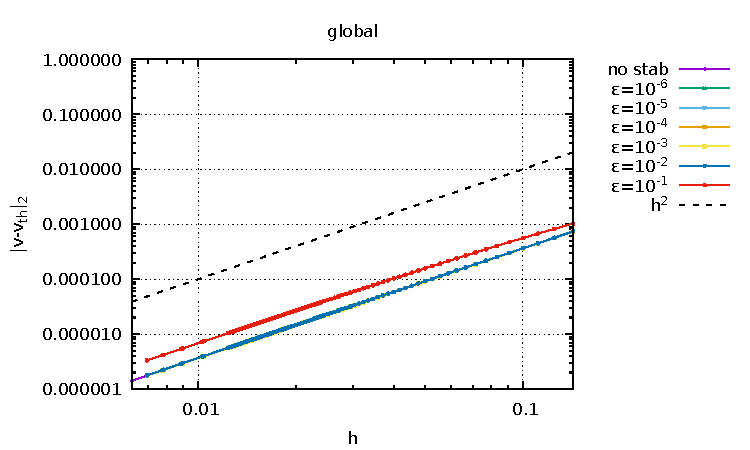
\includegraphics[width=8cm]{python_codes/fieldstone_115/results/errorsV_global.pdf}
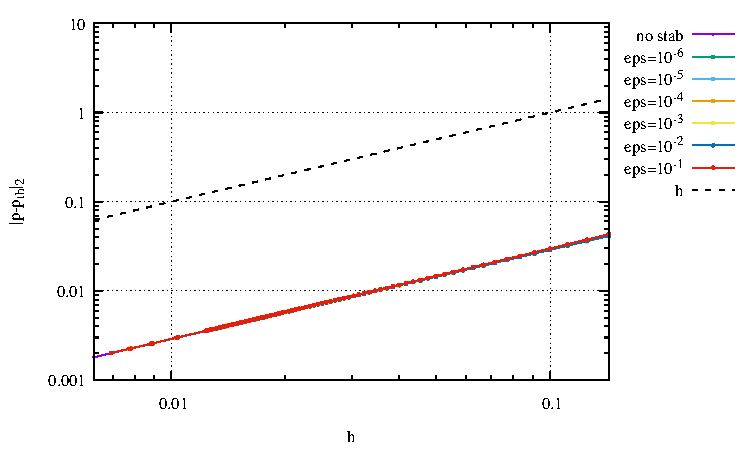
\includegraphics[width=8cm]{python_codes/fieldstone_115/results/errorsP_global.pdf}\\
{\captionfont Velocity and pressure errors as a function of the element size for meshes 6x6 to 128x128}
\end{center}


%-------------------------------------------
\subsection*{Local stabilisation}

\begin{center}
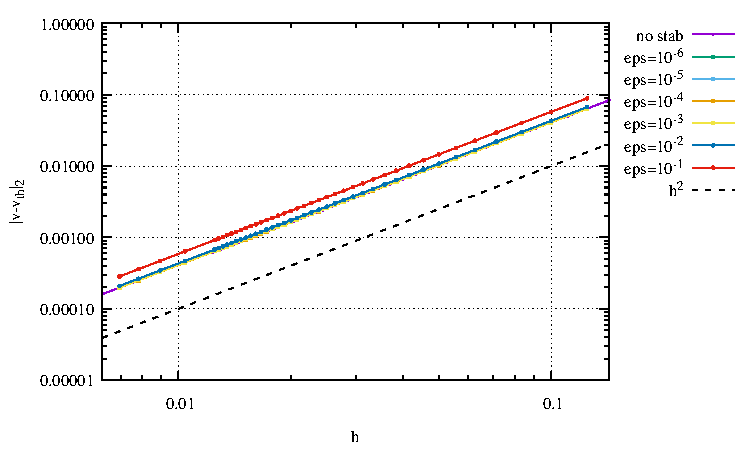
\includegraphics[width=8cm]{python_codes/fieldstone_115/results/errorsV_local.pdf}
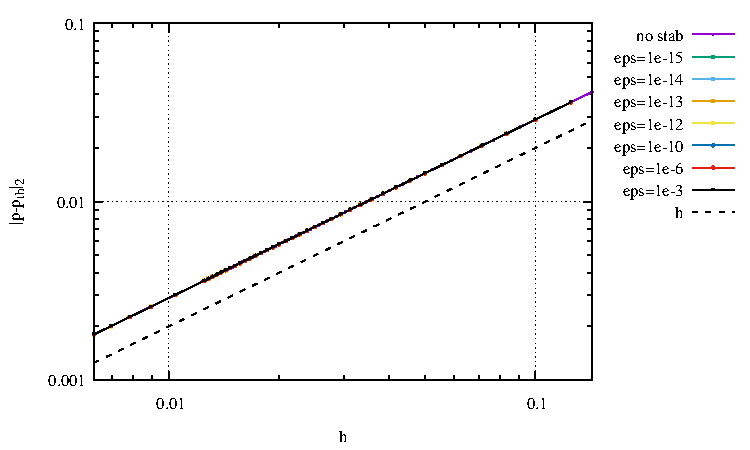
\includegraphics[width=8cm]{python_codes/fieldstone_115/results/errorsP_local.pdf}\\
{\captionfont Velocity and pressure errors as a function of the element size for meshes 6x6 to 128x128.
Only even numbers are allowed.}
\end{center}


%-------------------------------------------
\subsection*{Local stabilisation}




